\documentclass[10pt,a4paper]{article}
\usepackage[utf8]{inputenc}

\usepackage[landscape,margin=1cm]{geometry}
\usepackage[italian]{babel}
\usepackage{xcolor}
\usepackage{listings}
\usepackage{amsfonts} 
\usepackage{amssymb}

\usepackage{xparse}

\NewDocumentCommand{\codeword}{v}{%
\texttt{\textcolor{black}{#1}}%
}

\lstset{language=C,keywordstyle={\bfseries \color{black}}}


% colour themes to come. KnitR?

%-------------------------

\title{Formulario di Modelli di Calcolo e Algoritmi Avanzati}
\author{Paolo Speziali}
\date{Giugno 2022}
\usepackage[default]{raleway}
\usepackage{fontawesome}
\usepackage[T1]{fontenc}

\usepackage{hyperref}
\usepackage{enumitem}
\usepackage{lipsum}

\usepackage{xcolor}
\definecolor{customcolor}{HTML}{616AC5}
\definecolor{alert}{HTML}{CD5C5C}
\definecolor{w3schools}{HTML}{4CAF50}
\definecolor{subbox}{gray}{0.60}
\definecolor{codecolor}{HTML}{FFC300}
\colorlet{xx}{customcolor}


%--------------------------Editor mode.

\usepackage
[citestyle=authoryear,
sorting=nty,	  		%Sorts bibliography by year, name, title
autocite=footnote, 		%Autocite command generates footnotes
autolang=hyphen, 		
mincrossrefs=1, 	
backend=biber]
{biblatex}

\DeclareFieldFormat{postnote}{#1}
\DeclareFieldFormat{multipostnote}{#1}
\DeclareAutoCiteCommand{footnote}[f]{\footcite}{\footcites}

\bibliography{literature}
%----------------------------------------
%--------------------------------------------------------------------------------
\usepackage{tcolorbox}

\tcbuselibrary{most,listingsutf8,minted}

\tcbset{tcbox width=auto,left=1mm,top=1mm,bottom=1mm,
right=1mm,boxsep=1mm,middle=1pt}

\newenvironment{mycolorbox}[2]{%
\begin{tcolorbox}[grow to left by=-1em,grow to right by=-1em,capture=minipage,fonttitle=\large\bfseries, enhanced jigsaw,boxsep=1mm,colback=#1!30!white,on line,tcbox width=auto, toptitle=0mm,colframe=#1,opacityback=0.7,nobeforeafter,title=#2]%
}{\end{tcolorbox}\\[0.2em]}

\newenvironment{subbox}[2]{%
\begin{tcolorbox}[capture=minipage,fonttitle=\normalsize\bfseries, enhanced jigsaw,boxsep=1mm,colback=#1!30!white,on line,tcbox width=auto,left=0.3em,top=1mm, toptitle=0mm,colframe=#1,opacityback=0.7,nobeforeafter,title=#2]\footnotesize %
}{\normalsize\end{tcolorbox}\vspace{0.1em}}

\newenvironment{multibox}[1]{%
\begin{tcbraster}[raster columns=#1,raster equal height,nobeforeafter,raster column skip=1em,raster left skip=1em,raster right skip=1em]}{\end{tcbraster}}

\newenvironment{textbox}[1]{\begin{mycolorbox}{customcolor}{#1}}{\end{mycolorbox}}

%-------------------------------
\newtcblisting{codebox}[2]{colback=codecolor!5,colframe=codecolor!80!black,listing only, 
minted options={numbers=left,style=tcblatex,fontsize=\tiny,breaklines,autogobble,linenos,numbersep=3mm},
left=5mm,enhanced,
title=#2, fonttitle=\bfseries,
listing engine=minted,minted language=#1}

%--------------------------------------------------------------------------------
\newcommand{\punkti}{~\lbrack\dots\rbrack~}

\renewenvironment{quote}
               {\list{\faQuoteLeft\phantom{ }}{\rightmargin\leftmargin}%
                \item\relax\scriptsize\ignorespaces}
               {\unskip\unskip\phantom{xx}\faQuoteRight\endlist}
               

%--------------------------------------------------------------------------------
\newcommand{\bgupper}[3]{\colorbox{#1}{\color{#2}\huge\bfseries\MakeUppercase{#3}}}
\newcommand{\bg}[3]{\colorbox{#1}{\bfseries\color{#2}#3}}

\newcommand{\mycommand}[2]{{\ttfamily\detokenize{#1}}~\dotfill{}~{\footnotesize #2}\\}
\newcommand{\sep}{{\scriptsize~\faCircle{ }~}}


\newcommand{\bggreen}[1]{\medskip\bgupper{w3schools}{black}{#1}\\[0.5em]}
\newcommand{\green}[1]{\smallskip\bg{w3schools}{white}{#1}\\}
\newcommand{\red}[1]{\smallskip\bg{alert}{white}{#1}\\}

\usepackage{multicol}
\setlength{\columnsep}{30pt}

\setlength{\parindent}{0pt}
\pagestyle{empty}

\usepackage{csquotes}

\newcommand{\loremipsum}{Lorem ipsum dolor sit amet.}

\tolerance=1
\emergencystretch=\maxdimen
\hyphenpenalty=10000
\hbadness=10000


%--------------------------------------------------------------------------------
\begin{document}
\small
\begin{multicols}{3}

\maketitle
\thispagestyle{empty}


\section{Grammatiche}


\begin{textbox}{Tipi di grammatiche}

\red{Tipo 0}
Detta anche \textbf{non limitata}, ammette \textbf{qualunque tipo}
di produzione, anche quelle che accorciano le forme di
frase, come ad esempio quelle che si ottengono da \(\varepsilon\)-produzioni
(es. \(aA\,\rightarrow\,b\,|\,\varepsilon\)).

\red{Tipo 1}
Detta anche \textbf{context-sensitive}, ammette \textbf{qualunque tipo}
di produzione che \textbf{non accorci} le forme di frase
(es. \(aA\,\rightarrow\,Bb\)).

\red{Tipo 2}
Detta anche \textbf{context-free}, ammette produzioni in cui
il termine sinistro è formato da un solo non terminale
e la forma di frase non si accorcia mai \\
(es. \(A\,\rightarrow\,aBb\)).

\red{Tipo 3}
Detta anche \textbf{regolare}, ammette produzioni in cui
il termine sinistro è formato da un solo non terminale
e il termine destro o da un solo terminale o da un
terminale seguito da un non terminale\\
(es. \(A\,\rightarrow\,b\,|\,aB\)).

\end{textbox}

\section{Macchine a Registri}

\begin{textbox}{Operandi ed etichette}
Ogni operando \codeword{<op>} può avere una delle forme seguenti:
\begin{itemize}[leftmargin=*]
    \item \textbf{n}: \codeword{<op>} indica l’intero memorizzato nel registro n;
    \item \textbf{(n)}: \codeword{<op>} indica l’intero memorizzato nel registro indirizzato dal
    registro n;
    \item \textbf{\#n}: \codeword{<op>} indica il numero n.
\end{itemize}
Ogni etichetta \codeword{<et>} ha la forma \textbf{n}, ed indica il numero intero n.
\end{textbox}

\begin{textbox}{Istruzioni di trasferimento}
\begin{itemize}[leftmargin=*]
    \item \textbf{LOAD} <op>\quad(\codeword{R[0] := <op>});
    \item \textbf{STORE} <op>\quad(\codeword{R[<op>] := R[0]}).
\end{itemize}
\end{textbox}

\begin{textbox}{Istruzioni aritmetiche}
\begin{itemize}[leftmargin=*]
    \item \textbf{ADD} <op>\quad(\codeword{R[0] := R[0] + <op>});
    \item \textbf{SUB} <op>\quad(\codeword{R[0] := R[0] - <op>});
    \item \textbf{MULT} <op>\quad(\codeword{R[0] := R[0] * <op>});
    \item \textbf{DIV} <op>\quad(\codeword{R[0] := R[0] / <op>}).
\end{itemize}
\end{textbox}

\begin{textbox}{Istruzioni di I/O}
\begin{itemize}[leftmargin=*]
    \item \textbf{READ} <op>\quad(\codeword{R[<op>] := IN});
    \item \textbf{WRITE} <op>\quad(\codeword{OUT := <op>}).
\end{itemize}
\end{textbox}

\begin{textbox}{Istruzioni di salto e di controllo}
\begin{itemize}[leftmargin=*]
    \item \textbf{JUMP} <et>\quad(\codeword{CI := <et>});
    \item \textbf{JGTZ} <et>\quad(\codeword{if (R[0] > 0) then CI := <et> else CI := CI + 1});
    \item \textbf{JZERO} <et>\quad(\codeword{if (R[0] = 0) then CI := <et> else CI := CI + 1});
    \item \textbf{HALT}\quad(\codeword{fine, il calcolo si arresta}).
\end{itemize}
\end{textbox}

\section{Linguaggi}

\begin{textbox}{Pumping Lemma per L. Regolari}
Se L è un linguaggio regolare allora \\
\(\exists \, n \, > \, 0\) tale che \(\forall \, z \, \in \, L \) e
\(|z| \, \geq \, n\),\\si ha che
\(\exists \, u \, ,v \, ,w\) tali che:
\begin{enumerate}[leftmargin=*]
    \item \(z\, =\, uvw\)
    \item \(|uv|\, \leq\,  n\)
    \item \(|v|\, \geq\,  1\)
    \item \(uv^iw\,\in\,L,\,\forall\,i\,\geq\,0\)
\end{enumerate}

\end{textbox}

\begin{textbox}{Da Gram. Reg. a Esp. Reg.}
Dal sistema di equazioni lineari si ricava una espressione regolare
applicando le due tecniche seguenti ripetutamente:
\begin{itemize}[leftmargin=*]
    \item \textbf{Sostituzione}: si può sostituire un simbolo non terminale con una espressione equivalente \\
    (es. \(A\, aB\, +\, b,\, B\, =\, cA\,\Rightarrow \,  =\, acA\, +\, b)\)
    \item \textbf{Eliminazione della ricorsione}: si può sostituire la prima equazione con la seconda\\
    \(A\,=\,\alpha_1A\,+\,\alpha_2A\,+\,...\,+\
    \alpha_nA\,+\,\beta_1\,+\,\beta_2\,+\,...\,+\
    \beta_n\) \\
    \(A\,=\,(\alpha_1\,+\,\alpha_2\,+\,...\,+\
    \alpha_n\,)^\ast(\beta_1\,+\,\beta_2\,+\,...\,+\
    \beta_n)\)
\end{itemize}

\end{textbox}

\begin{textbox}{Forma ridotta}
Una grammatica G CF è in forma ridotta se:
\begin{itemize}[leftmargin=*]
    \item G non contiene \(\varepsilon\)-produzioni
    se non sull’assioma, ed in tal caso l’assioma non
    compare a destra di nessuna produzione;
    \item G non contiene simboli inutili, cioè non fecondi o non generabili;
    \item G non contiene produzioni unitarie\\(cioè del tipo \(A\,\rightarrow\,B\)).
\end{itemize}

\end{textbox}

\begin{textbox}{Forma normale di Greibach (GNF)}
Una grammatica G CF è in GNF se tutte le sue produzioni sono del tipo \(A\,\rightarrow\,a\beta\), dove \(\beta\) è una sequenza (eventualmente vuota) di non terminali e \(a\)  è un simbolo terminale.
\end{textbox}

\begin{textbox}{Forma normale di Chomsky (CNF)}
Una grammatica G CF è in CNF se tutte le sue produzioni sono del tipo \(A\,\rightarrow\,BC\) o \(A\,\rightarrow\,a\).\\
Per arrivarci si porta G in forma ridotta e si sostituisce ogni terminale \(a\) con un non terminale \(X_a\) in tutte le produzioni
in cui compare \(a\) ed si introduce la produzione \(X_a\,\rightarrow\,a\)
(la forma ottenuta a questo punto si chiama \textbf{quasi CFN}).\\
Infine si sotituisce ricorsivamente ogni produzione del tipo:\\
\(A\,\rightarrow\,BC\alpha\) con le seguenti:
\(A\,\rightarrow\,BD\), \(D\,\rightarrow\,C\alpha\) dove D è un nuovo non terminale.
\end{textbox}

\begin{textbox}{Pumping Lemma per L CF}
Se L è un linguaggio CF allora \\
\(\exists \, n \, > \, 0\) tale che \(\forall \, z \, \in \, L \) e
\(|z| \, \geq \, n\),\\si ha che
\(\exists \, u \, ,v \, ,w \, ,x \, ,y\) tali che:
\begin{enumerate}[leftmargin=*]
    \item \(z\, =\, uvwxy\)
    \item \(|vwx|\, \leq\,  n\)
    \item \(|vx|\, \geq\,  1\)
    \item \(uv^iwx^iy\,\in\,L,\,\forall\,i\,\geq\,0\)
\end{enumerate}
\end{textbox}

%--------------------------------------------------------------

\section{Trattabilità}

\begin{textbox}{Problemi in NP}
Dimostrare che un problema \(B\) appartiene ad NP:
\begin{enumerate}[leftmargin=*]
    \item Definire in cosa consiste l'insieme \(S\) delle \textbf{soluzioni candidate} di \(B\) e quale è la proprietà che ogni soluzione candidata deve possedere per essere una soluzione effettiva;
    \item Definire uno \textbf{schema di codifica} delle soluzioni candidate di \(B\);
    \item Mostrare che le codifiche delle soluzioni candidate hanno \textbf{taglia polinomiale} nell'input;
    \item Definire un \textbf{algoritmo deterministico} che verifica in tempo polinomiale se una data soluzione candidata rispetta la proprietà richiesta.
\end{enumerate}
\end{textbox}


%--------------------------------------------------------------


\section{Complessità}

\begin{textbox}{Tipologie di problemi}
Per definire le varie tipologie di problemi useremo degli esempi che
partono dal concetto di \textbf{Clique}.\\

\begin{textbox}{Problemi di decisione}
Un problema di decisione \(P_D\) è definito da:
\begin{itemize}[leftmargin=*]
    \item Un insieme di istanze \(I_{P_D}\);
    \item Un predicato \(\pi\): \(I_{P_D} \rightarrow\) \{vero, falso\}.
\end{itemize}

\codeword{CLIQUE}\\
\codeword{Istanza}: Grafo \(G\), intero \(K > 0\) \\
\codeword{Predicato}: Esiste una clique di \(G\) di dimensione \(\geq\) K ?

\end{textbox}

\begin{textbox}{Problemi di ricerca}
Un problema di decisione \(P_R\) è definito da:
\begin{itemize}[leftmargin=*]
    \item Un insieme di istanze \(I_{P_R}\);
    \item Un insieme di soluzioni candidate  \(S_{P_R}\);
    \item Una proprietà di ammissibilità che deve valere per ogni soluzione di una
    data istanza.
\end{itemize}

\codeword{RICERCA CLIQUE}\\
\codeword{Istanza}: Grafo \(G\), intero \(K > 0\) \\
\codeword{Soluzione candidata}: Sottoinsieme \(V'\) di vertici \\
\codeword{Ammissibilità}: \(V'\) è una clique di \(G\) di dimensione \(\geq\) K

Un algoritmo che lo risolve prende in input una
istanza \(x\) e restituisce (se esiste) un elemento di\\
\(Sol(x)\) = \{ \(y\,\in\,S_{P_R}\) : \(y\) rispetta la proprietà di ammissibilità \}.

\end{textbox}

\end{textbox}

\begin{textbox}{Tipologie di problemi}

Ogni problema di ricerca \(P_R\) ha un problema di decisione associato \(P_D\).\\

\begin{textbox}{Problemi di enumerazione}
Un problema di decisione \(P_E\) è definito da:
\begin{itemize}[leftmargin=*]
    \item Un insieme di istanze \(I_{P_E}\);
    \item Un insieme di soluzioni candidate  \(S_{P_E}\);
    \item Una proprietà di ammissibilità.
\end{itemize}
Un algoritmo che lo risolve prende in input una istanza \(x\)  e
restituisce la cardinalità dell’insieme \(Sol(x)\).
\end{textbox}

\begin{textbox}{Problemi di ottimizzazione}
Un problema di decisione \(P_E\) è definito da:
\begin{itemize}[leftmargin=*]
    \item Un insieme di istanze \(I_{P_O}\), un insieme di soluzioni candidate  \(S{P_O}\), ed una proprietà di ammissibilità;
    \item Una funzione di misura \\\(\mu:\,I_{P_O}\,\times S_{P_O}\,\rightarrow\,\mathbb{N} \)
    definita solo sulle coppie \((x,y)\) tali che \(y\,\in\,Sol(x)\);
    \item Un criterio di scelta \(c\,\in\,\)\{MIN, MAX\};
\end{itemize}
Un algoritmo che lo risolve prende
una istanza \(x\) e restituisce \(y\) tale
che,\\ \(\forall\,z\,\in\,Sol(x)\), \\
\(m(x,y) \leq m(x,z)\) se \(c\) = MIN e \\
\(m(x,y) \geq m(x,z)\) se \(c\) = MAX.\\
\codeword{MASSIMA CLIQUE}\\
\codeword{Istanza}: Grafo \(G\)\\
\codeword{Soluzione candidata}: Insieme \(V'\) di vertici \\
\codeword{Ammissibilità}: \(V'\) è una clique di \(G\)\\
\codeword{Misura}: \(|V'|\) \\
\codeword{Criterio}: MAX
\end{textbox}

\end{textbox}


%--------------------------------------------------------------


\section{Complessità parametrica}

\begin{textbox}{Problema parametrizzato}
Si tratta di un linguaggio \(L \subseteq \Sigma^\ast \times \mathbb{N}\).
Data un’istanza \((x,k) \in \Sigma^\ast \times \mathbb{N}\), \(k\) è
il \textbf{parametro} del problema.

\(L\) è detto Fixed-Parameter Tractable (\textbf{FPT}) se esiste una terna \((A,f,c)\) dove:
\begin{itemize}[leftmargin=*]
    \item \(f:\mathbb{N} \rightarrow \mathbb{N}\) è una funzione calcolabile;
    \item \(c\) è una costante;
    \item \(A\) è un algoritmo che decide se una data istanza \((x,k)\) appartiene ad \(L\) in un tempo limitato superiormente da \(f(k)\cdot|x|^c\).
\end{itemize}

\(L\) è detto Slice-Wise Polynomial (\textbf{XP}) se esiste una terna \((A,f,g)\) dove:
\begin{itemize}[leftmargin=*]
    \item \(f, g:\mathbb{N} \rightarrow \mathbb{N}\) sono due funzioni calcolabili;
    \item \(A\) è un algoritmo che decide se una data istanza \((x,k)\) appartiene ad \(L\) in un tempo limitato superiormente da \(f(k)\cdot|x|^{g(k)}\).
\end{itemize}
\end{textbox}

\begin{textbox}{Kernelizzazione}
Approccio sistematico allo studio di
algoritmi di preprocessing che lavorano in
tempo polinomiale.

Sia  \(Q \subseteq \Sigma^\ast \times \mathbb{N}\) un problema parametrizzato, diciamo che due
istanze \((x,k)\) e \((x',k')\) sono equivalenti se  \((x,k)\in Q \Leftrightarrow (x',k')\in Q \).

Una funzione \(\Phi: \Sigma^\ast \times \mathbb{N} \rightarrow \Sigma^\ast \times \mathbb{N}\) è una \textbf{regola di riduzione} per \(Q\) se:
\begin{itemize}[leftmargin=*]
    \item \(\Phi\) mappa ciascuna istanza \((x,k)\) in una equivalente \((x',k')\), ovvero è \textbf{safe};
    \item \(\Phi\) è calcolabile in tempo polinomiale nella dimensione di \((x,k)\).
\end{itemize}

La \textbf{dimensione dell’output} di \(A\) è
una funzione \(size_A(k):\mathbb{N} \rightarrow \mathbb{N}\cup\{\infty\}\)
definita come segue:\\
\(size_A(k) = sup\{|x'|+k': (x',k') = A(x,k), x \in \Sigma^\ast\}\).

Un \textbf{algoritmo di kernelizzazione} \(A\) per il problema \(Q\) è un algoritmo di
preelaborazione tale che \(size_A(k) \leq g(k)\), per una qualche
funzione calcolabile \(g:\mathbb{N} \rightarrow \mathbb{N}\).
Se la funzione g è \textbf{polinomiale} (\textbf{lineare}) in k, allora diciamo che Q ammette un
\textbf{kernel polinomiale} (\textbf{lineare}).

Un problema parametrizzato Q \textbf{è FPT} se e solo se
\textbf{ammette un algoritmo di kernelizzazione}.
\end{textbox}

\begin{textbox}{Matching}
Dato un grafo bipartito \(G=(X\cup Y,E)\), un \textbf{matching} di \(X\) in \(Y\) è un
insieme \(M\subseteq E\) di archi indipendenti tale che ciascun vertice di \(X\) è
adiacente ad un arco di \(M\).

Per un qualsiasi sottoinsieme \(C\subseteq X\), sia \(N(C)\) l’insieme di vertici in
\(Y\) adiacenti ai vertici in \(C\).

I seguenti teoremi rappresentano strumenti fondamentali
nell’ambito della kernelizzazione:
\begin{itemize}[leftmargin=*]
    \item La \textbf{dimensione minima di un vertex cover} in un grafo bipartito è pari alla \textbf{dimensione del massimo matching}.
    \item Sia \(G\) un grafo bipartito. Allora \(G\) \textbf{contiene un matching} di \(X\) in \(Y\) se e solo se \(|N(C)|\geq |C|\) per ogni sottoinsieme \(C\subseteq X\).
    \item Sia \(G\) un grafo bipartito. Possiamo trovare un matching di dimensione massima
    (e un vertex cover di dimensione minima) in PTIME. 
    
    Inoltre, in tempo polinomiale, possiamo trovare o un matching di 
    \(X\) in \(Y\), oppure un insieme minimale non vuoto \(C\subseteq X\) tale che \(|N(C)|<|C|\).
\end{itemize}
\end{textbox}

\begin{textbox}{Crown Decomposition}
Una crown decomposition di un grafo \(G=(V,E)\) è una partizione di
\(V\) in tre insiemi \((C,H,R)\) tale che:
\begin{itemize}[leftmargin=*]
    \item \(C\) è un \textbf{indipendent set non vuoto};
    \item Nessun vertice di \(C\) è connesso a un vertice di R, ovvero \textbf{H separa C e R};
    \item \(E\) \textbf{contiene un matching} di \(H\) in \(C\). 
\end{itemize}
\vspace{-15pt}
\begin{figure}[H]
    \centering
    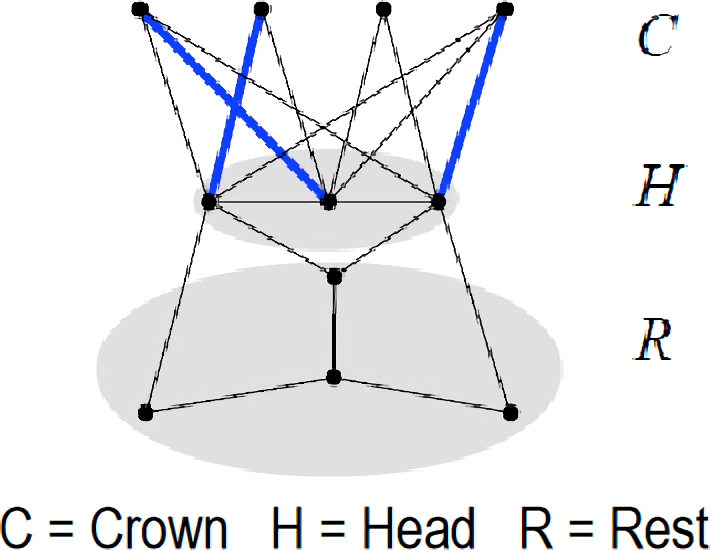
\includegraphics[width=0.5\textwidth]{crown.png}
\end{figure}
\vspace{-15pt}
Sia \(G\) un grafo senza vertici isolati e con
almeno \(3k+1\) vertici. Allora \(G\) contiene
un \textbf{matching} di dimensione \(k+1\) oppure
una \textbf{crown decomposition}.
Inoltre, una delle due strutture può essere calcolata
in tempo polinomiale.
\end{textbox}

\begin{textbox}{Teoremi di Robertson-Seymour}
Un grafo \(H\) è un \textbf{minor} di \(G\), denotato con \(H \leq_M G\), se \(H\)
può essere ottenuto da un sottografo di \(G\) attraverso una serie di
contrazioni di un arco (o con rimozione di un arco o un vertice).

Una famiglia di grafi \(F\) è \textbf{minor-closed}, se per ogni grafo \(G \in F\) e
per ogni minore \(H\) di \(G\), abbiamo che \(H \in F\).

\(\forall k\) fissato, la famiglia di grafi con vertex cover
number al più \(k\) è minor-closed.

\begin{enumerate}[leftmargin=*]
    \item Qualsiasi famiglia infinita di grafi contiene due elementi tali che uno è un minore dell’altro.
    
    Per ogni fissata famiglia minor-closed \(F\), esiste un insieme finito di grafi \(Forb(F)\), detta famiglia dei \textbf{minimal forbidden minors}, tale che qualsiasi grafo \(G\) appartiene a \(F\) se e solo se non esiste un minor di \(G\) che corrisponde (a meno di un isomorfismo) a un membro di \(Forb(F)\).
    \item Esiste una funzione calcolabile \(f\) e un algoritmo \(A\), tali che per una data coppia di grafi\\\(H=(V’,E’)\) e \(G=(V,E)\), \(A\) decide se \(H \leq_M G\) in tempo \(f(|H|)\cdot |V|^3\).
    \item Sia \(F\) una famiglia di grafi minor-closed, esiste una costante \(c_F\) che dipende soltanto da \(F\), tale che per ogni grafo \(G\) con \(n\) vertici, possiamo decidere se \(G\in F\) in tempo al più \(c_F\cdot n^3\).
    \item Per ogni fissato \(k\), esiste un algoritmo che risolve \codeword{VERTEX-COVER} in tempo \(c_k\cdot n^3\) dove \(c_k=f(k)\) per una qualche funzione calcolabile \(f\).
\end{enumerate}
L'ultimo teorema non ci dimostra che \codeword{VERTEX-COVER} è FPT, 
ci dice però che esiste una collezione di algoritmi FPT per
il nostro problema, uno per ogni valore di \(k\).

Un problema parametrizzato L è detto \textbf{nonuniformly FPT}
se esiste una terna \(((A_K)_{K\in \mathbb{N}},f,c)\) dove:
\begin{itemize}[leftmargin=*]
    \item \(f:\mathbb{N} \rightarrow \mathbb{N}\) è una funzione calcolabile;
    \item \(c\) è una costante;
    \item \((A_K)_{K\in \mathbb{N}}\) è una collezione di algoritmi, tale che
    \(\forall k \in \mathbb{N}\), \(A_k\) decide se una data istanza \((x,k)\)
    appartiene ad \(L\) in un tempo limitato da \(f(k)\cdot |x|^c\).
\end{itemize}
\end{textbox}

\begin{textbox}{Treewidth}
Se un grafo ha un valore di treewidth
piccolo, allora possiamo applicare un approccio di
programmazione dinamica simile a quello usato per gli alberi.

Una \textbf{tree decomposition} di \(G=(V,E)\) è una coppia \(\tau=(T, \{X_t\}_{t\in T})\) tale che:
\begin{itemize}[leftmargin=*]
    \item \(T\) è un albero e ciascun nodo \(t\in T\) è associato con un un insieme \(X_t \subseteq V\) chiamato \textbf{bag};
    \item \(\bigcup_{t\in T}X_t=V\) (per ciascun vertice di G esiste almeno una bag che lo contiene);
    \item \(\forall (u,v) \in E\), \(\exists\) un nodo \(t\in T\) tale che \(\{u,v\} \subseteq X_t\)
    (per ciascun arco di G esiste almeno una bag che contiene entrambi i suoi estremi);
    \item \(\forall u \in V\), \(T_u = \{t\in T: u\in X_t\}\) induce un sottoalbero connesso di \(T\).
\end{itemize}

La \textbf{width} di \(\tau=(T, \{X_t\}_{t\in T})\) è pari alla dimensione della bag più
grande meno uno, ovvero:\\\(width(\tau) = max_{t\in T} |X_t|-1\).

La \textbf{treewidth} di un grafo \(G\), denotata \(tw(G)\), è la più piccola width
possibile per una sua tree decomposition.

Una tree decomposition \(\tau\) di \(G\) è \textbf{nice} se le seguenti
proprietà valgono, assumendo che \(T\) è radicato nel nodo \(r\):
\begin{itemize}[leftmargin=*]
    \item \(X_r=\varnothing\) e \(X_l=\varnothing\) per ogni foglia l di T.
    \item Per ogni nodo interno t di T, vale una delle seguenti proprietà:
    \begin{enumerate}[leftmargin=*]
        \item \textbf{Introduce node}: \(t\) ha solo un figlio \(t'\) in \(T\) tale che
        \(X_t = X_{t'}\bigcup \{v\}\) per un qualche vertice \(v \notin X_{t'}\).
        Diciamo che \(v\) è introdotto in \(t\).
        \item \textbf{Forget node}: \(t\) ha solo un figlio \(t'\) in \(T\) tale che
        \(X_t\bigcup \{w\} = X_{t'}\) per un qualche vertice \(w \in X_{t'}\).
        Diciamo che \(w\) è dimenticato in \(t\).
        \item \textbf{Join node}: \(t\) ha solo due figli \(t_1\) e \(t_1\) in \(T\) tale che
        \(X_t = X_{t_1}= X_{t_2}\).
    \end{enumerate}
\end{itemize}

Se un grafo \(G\) ammette una tree decomposition
\(\tau\) con width al più \(k\), allora ammette anche una nice
tree decomposition \(\tau'\) con width al più \(k\) e tale che
\(|T’|\in O(k|V|)\).

Inoltre, \(\tau'\) è calcolabile partendo da \(\tau\) in tempo \(O(k^2\cdot max(|T|, |V|)).\)
\end{textbox}



\begin{textbox}{Path decomposition}
Una tree decomposition \(\mathrm{P}=(P, {X_t}_{t\in P})\) in cui \(P\) è un cammino,
prende il nome di \textbf{path decomposition}.

La \textbf{width} di \(\mathrm{P}=(P, {X_t}_{t\in P})\) è ancora pari alla dimensione della bag
più grande meno uno, ovvero: \(width(\mathrm{P}) = max_{t\in P} |X_t|-1\).

La \textbf{pathwidth} di un grafo \(G\), denotata \(pw(G)\), è la più piccola width
possibile per una sua path decomposition.

Per definizione, dato un qualsiasi grafo \(G\), abbiamo che \(tw(G)\leq pw(G)\).

Una \textbf{nice path decomposition} può essere definita similmente a una nice
tree decomposition, ignorando il concetto di join node.
\end{textbox}

\begin{textbox}{Calcolo della treewidth}
Sia \(G\) un grafo con \(n\) vertici e sia \(k\)
un intero positivo. Esiste un algoritmo che, in tempo \(O(k^{O(k^3)}\cdot n)\), o
calcola una tree decomposition di \(G\) con width al più \(k\), oppure
termina concludendo che \(tw(G)>k\).
\end{textbox}


\begin{textbox}{W-hierarchy}
Uno strumento utile al fine di identificare quali sono i problemi
intrattabili a parametro fissato (se quindi ammettono algoritmi FPT) è la \textbf{W-hierarchy}.

Siano \(A, B\) due problemi parametrizzati. Una riduzione
parametrizzata da \(A\) a \(B\) è un algoritmo che, per ogni data
istanza \((x,k)\) di \(A\), fornisce in output un’istanza \((x’,k’)\) di \(B\) tale che:
\begin{enumerate}[leftmargin=*]
    \item \((x,k) \in A\) se e solo se \((x’,k’) \in B\), ovvero le due istanze sono equivalenti;
    \item \(k’ \leq g(k)\), dove \(g\) è una qualche funzione;
    \item \((x’,k’)\) è calcolata in tempo \(f(k)\cdot |x|^{O(1)}\), dove \(f\) è una qualche funzione calcolabile.
\end{enumerate}
Se esiste una riduzione parametrizzata da \(A\) a \(B\), e \(B\) è un problema
FPT, allora \(A\) è un problema FPT.
Se ne esiste un'altra \(B\) a \(C\), altro problema paramterizzato, allora esiste una riduzione parametrizzata da \(A\) a \(C\).
\end{textbox}

\begin{textbox}{Circuiti Booleani}
Un \textbf{circuito booleano} è un grafo diretto aciclico dove ogni nodo v
è etichettato come segue:
\begin{itemize}[leftmargin=*]
    \item v è un nodo di \textbf{input} se il suo indegree è \(0\);
    \item v è un nodo di \textbf{negazione} se il suo indegree è \(1\);
    \item v è un nodo di \textbf{and} o di \textbf{or} se il suo indegree è almeno \(2\)
\end{itemize}
Inoltre esiste esattamente un nodo con outdegree \(0\) etichettato
come nodo di \textbf{output}.

Dato un circuito booleano, assegnando un valore in \(\{0,1\}\) a
ciascun nodo di input e applicando gli operatori logici
corrispondenti alle etichette dei nodi del circuito, otteniamo un
valore in \(\{0,1\}\) per il nodo in output.
Se tale valore è \(1\) allora diciamo che l’assegnamento in input
soddisfa il circuito.
Verificare se un dato assegnamento soddisfa o meno un
circuito è fattibile in tempo polinomiale nella dimensione del
circuito.

Sappiamo che decidere se un circuito booleano ammette un
assegnamento dell’input che lo soddisfa è
NP-completo.
Al fine di definire una versione parametrizzata del problema,
definiamo il \textbf{peso di un assegnamento} come il numero di nodi
in input a cui viene assegnato il valore \(1\).

Dato un circuito booleano \(C\) e un intero \(k\), il \codeword{WEIGHTED-CIRCUIT-SAT}
(\textbf{WCS}) è il problema di decidere se \(C\) ammette un
assegnamento che lo soddisfa con peso al più \(k\).
Se \(n\) è la dimensione del circuito, esistono \(O(n^k)\) possibili
assegnamenti, ognuno verificabile in tempo polinomiale,
pertanto WCS appartiene banalmente alla classe XP (si ritiene non sia FPT).

La \textbf{depth} di un circuito booleano è pari alla lunghezza
del più lungo cammino tra un nodo di input e il nodo di output.

La \textbf{weft} di un circuito booleano è pari al numero massimo
di nodi con indegree maggiore di \(2\) in un qualsiasi percorso da un
nodo di input al nodo di output.

Sia \(C_{t,d}\) la famiglia dei circuiti booleani con weft al più \(t\) e depth al
più \(d\), e sia WSC[\(C_{t,d}\)] la restrizione del problema WSC a questa
famiglia di circuiti.
Per un dato \(t \geq 1\), la classe W[t] è costituita da tutti i problemi
parametrizzati \(P\) per cui esiste una riduzione parametrizzata da \(P\) 
a WSC[\(C_{t,d}\)] per un qualche fissato valore di \(d \geq 1\).
\end{textbox}


%\begin{textbox}{Subboxes}
%---------------------------------------------
%\begin{multibox}{2} % number of boxes in a row
%\begin{subbox}{subbox}{test}

%\red{test} 
%\bggreen{test}
%\href{https://latex-ninja.com}{Link}
%\end{subbox}
%\begin{subbox}{customcolor}{test}
%\scriptsize


%\bggreen{test}
%\tiny
%super small font

%\mycommand{$\land$}{AND $\land$}
%\mycommand{$\lor$}{OR $\lor$}
%\end{subbox}
%\end{multibox}

%---------------------------------------------
%\begin{multibox}{2} % number of boxes in a row
%\begin{subbox}{subbox}{ Info}
%
%\red{bla}\\
%\bggreen{XX}\\

%\end{subbox}
%\begin{subbox}{customcolor}{Info}
%
%\end{subbox}
%\end{multibox}
%\end{textbox}

%---------------------------------------------
\end{multicols}

\end{document}
